
%\chapter{Tests and Results}
 \chapter{Teste și rezultate experimentale}
\label{cap:rezultate}

%Ponderea acestui capitol relativ la întreaga lucrare este de 5-10\%.
%
%Aici sunt prezentate metodele de validare a soluțiilor/sistemului descris în capitolele anterioare, scenariile de testare a corectitudinii funcționale, a utilizabilității, performanței etc.   
%
%Rezultatele testelor experimentale necesită, în general interpretări (dacă rezultatele obținute corespund așteptărilor, intuițiilor cititorului, de ce apar variații/excepții etc.) și comparații cu rezultatele altor metode similare. 
%
%Sistemele de testare și testele propriu-zise trebuie descrise detaliat astfel încât să poată fi reproduse și de alții care poate vor să-și compare soluțiile lor cu a voastră (eventual, codul testelor poate fi pus în anexe). Dacă se poate alegeți pentru evaluarea sistemului vostru benchmark-uri (pachete de testare) dedicate, astfel încât comparația cu alte sisteme să poată fi făcută mai ușor. În plus, astfel de teste sunt mult mai complete și mai realiste decât cele dezvoltate de voi. Oricum, încercați ca testele efectuate să nu fie triviale, ci să acopere scenarii cât mai reale, mai complexe și mai relevante ale funcționării sistemului vostru. 

%\section{Functional Tests}
 \section{Teste de funcționalitate}
 
În testarea sistemului s-a pus accentul pe testare celor două funcționalități de protecție împotrivă atacurilor de SQL injection și a utilizatorilor de Tor. 

Pentru testarea modelului folosit în prevenirea atacurilor de SQL injection s-a folosit setul de date de test specificat și în capitolul ~\ref{cap:implementare}. Acest set a fost obținut din setul inițial de date de antrenare, acesta fiind împărțit în 2 seturi separate cu proporția de 70\%(set antrenare) și respectiv 30\%(set testare). 
 
\begin{center}
	\begin{tabular}{||c c c c||} 
		\hline
		Tip set de testare  & Preziceri corecte & Dimensiune set & Acuratete(\%) \\ [0.5ex] 
		\hline\hline
		Clean \& infected & 187596 & 189278 & 99.11 \\ 
		\hline
		Clean & 5466 & 6258 & 87.34 \\
		\hline
		Infected & 182130 & 193020 & 99.51 \\
		\hline
	\end{tabular}
\end{center}

Pe baza tabelului de mai sus se pot observa diferențe majore de performanta între detecția pe setul "Clean" și pe "Infected". Aceste diferențe, respectiv scăderi de performanță în cazul setului Clean, se datorează dimensiunii mult mai mici a setului de Clean folosit și în antrenarea modelului. 

Pentru testarea eficienței sistemului de blocare a adreselor IP ale rețelei Tor, s-a realizat o referință între datele colectate de modulul de monitorizare a activității rețelei Tor. 

În prima diagrama este prezentată diferența procentuală dintre adresele IP cu un uptime mai mare de 7 zile în ultima lună și cele cu un uptime mai mic. În cea de a doua diagramă este evidențiată diferența dintre uptime-ul total ale acestor adrese IP din ultima lună. Printr-o analiză simplă în paralel a datelor din cele două diagrame, se poate observa că deși doar 20.31\% din IP-urile folosite de rețeaua Tor sunt blocate, din timpul total de uptime din ultima lună, 75.6\% aparține acestor adrese IP .

\begin{figure}
	\centering
	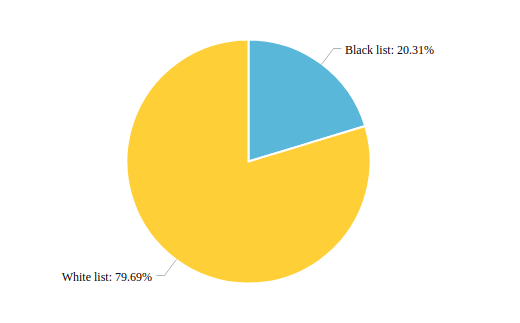
\includegraphics[width=0.7\textwidth]{test_case_1.png}
	\caption{ Raportul dintre numărul IP-urilor de pe Blacklist și Whitelist dintr-o lună }
	\label{fig:test_1}
\end{figure}

\begin{figure}
	\centering
	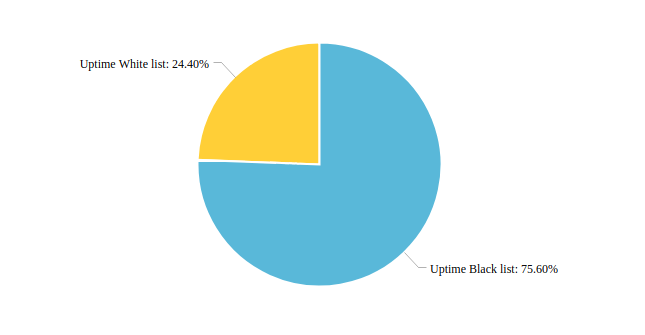
\includegraphics[width=0.7\textwidth]{test_case_2.png}
	\caption{ Raportul dintre uptime-ul IP-urile de pe Blacklist și Whitelist din aceeași lună }
	\label{fig:test_2}
\end{figure}


\newpage
%\section{Performance Tests}
 \section{Teste de performanță}

Sistemul propus a fost testat pe două configurații diferite pentru PC-ul gazdă: Intel Core i7-6600U CPU cu 4 nuclee și o frecvență de 2.6 GHz, cu 16 GB RAM DDR4 și i7-4790k CPU cu 4 nuclee și o frecvență maximă de 4.0 GHz, cu 16 GB RAM DDR4. Ambele sisteme furnizând mult mai multe resurse decât cele necesare unei funcționari optime. În cea ce privește resursele minime necesare, acestea trebuie să fie cele necesare rulării unui sistem de operare Windows 10: un procesor cu o frecvență mai mare de 1.0 GHz și o memorie mai mare sau egală cu 2 GB de RAM. În cea ce privește capacitățile sistemului de a suporta conexiuni exterioare, acesta nu a fost testat decât manual, prin intermediul unor mașini virtuale. 